%
\begin{simplebox}{Themen-Methodik}
%
Hier soll die Methode, welche zur Beantwortung der Fragestellung eingesetzt wird, ausführlich beschrieben werden.
Üblicherweise werden dazu folgende Themen behandelt:
%
\begin{itemize}
\item Festlegen von Bezeichnungen und Abbkürzungen 
\item Angabe der relevanten Formeln 
\item Beschreibung der verwendeten Software 
\item Beschreibung der verwendeten Programmiersprachen und Bibliotheken
\item Darstellung des Vorgehens mittels eines Flussdiagramms 
\end{itemize}
%
\end{simplebox}
%
Im Folgenden wird immer wieder auf das vorliegende Dokument Bezug genommen. 
Um hierbei Schreibaufwand zu sparen wird das vorliegende Dokument im weiteren Verlauf als \textit{Hilfestellung} bezeichnet
\par
Der prinzipielle Aufbau eines Abschnitts in der Hilfestellung ist in Abbildung \ref{fig:seite} zu sehen.
Der Abschnitt beginnt mit einem Kasten, indem die wichtigsten Punkte, welche in diesem Abschnitt behandelt werden sollen, aufgeführt sind.
Dabei kann es sein, dass manche der aufgelisteten Punkte in einem konkreten Fall nicht relevant sind.
So werden z.B. für die Hilfestellung keine Formeln benötigt, weswegen der entsprechende Punkt entfällt. 
%
\begin{figure}[h!]
\begin{tikzpicture}
\node[](fig) at (0,0){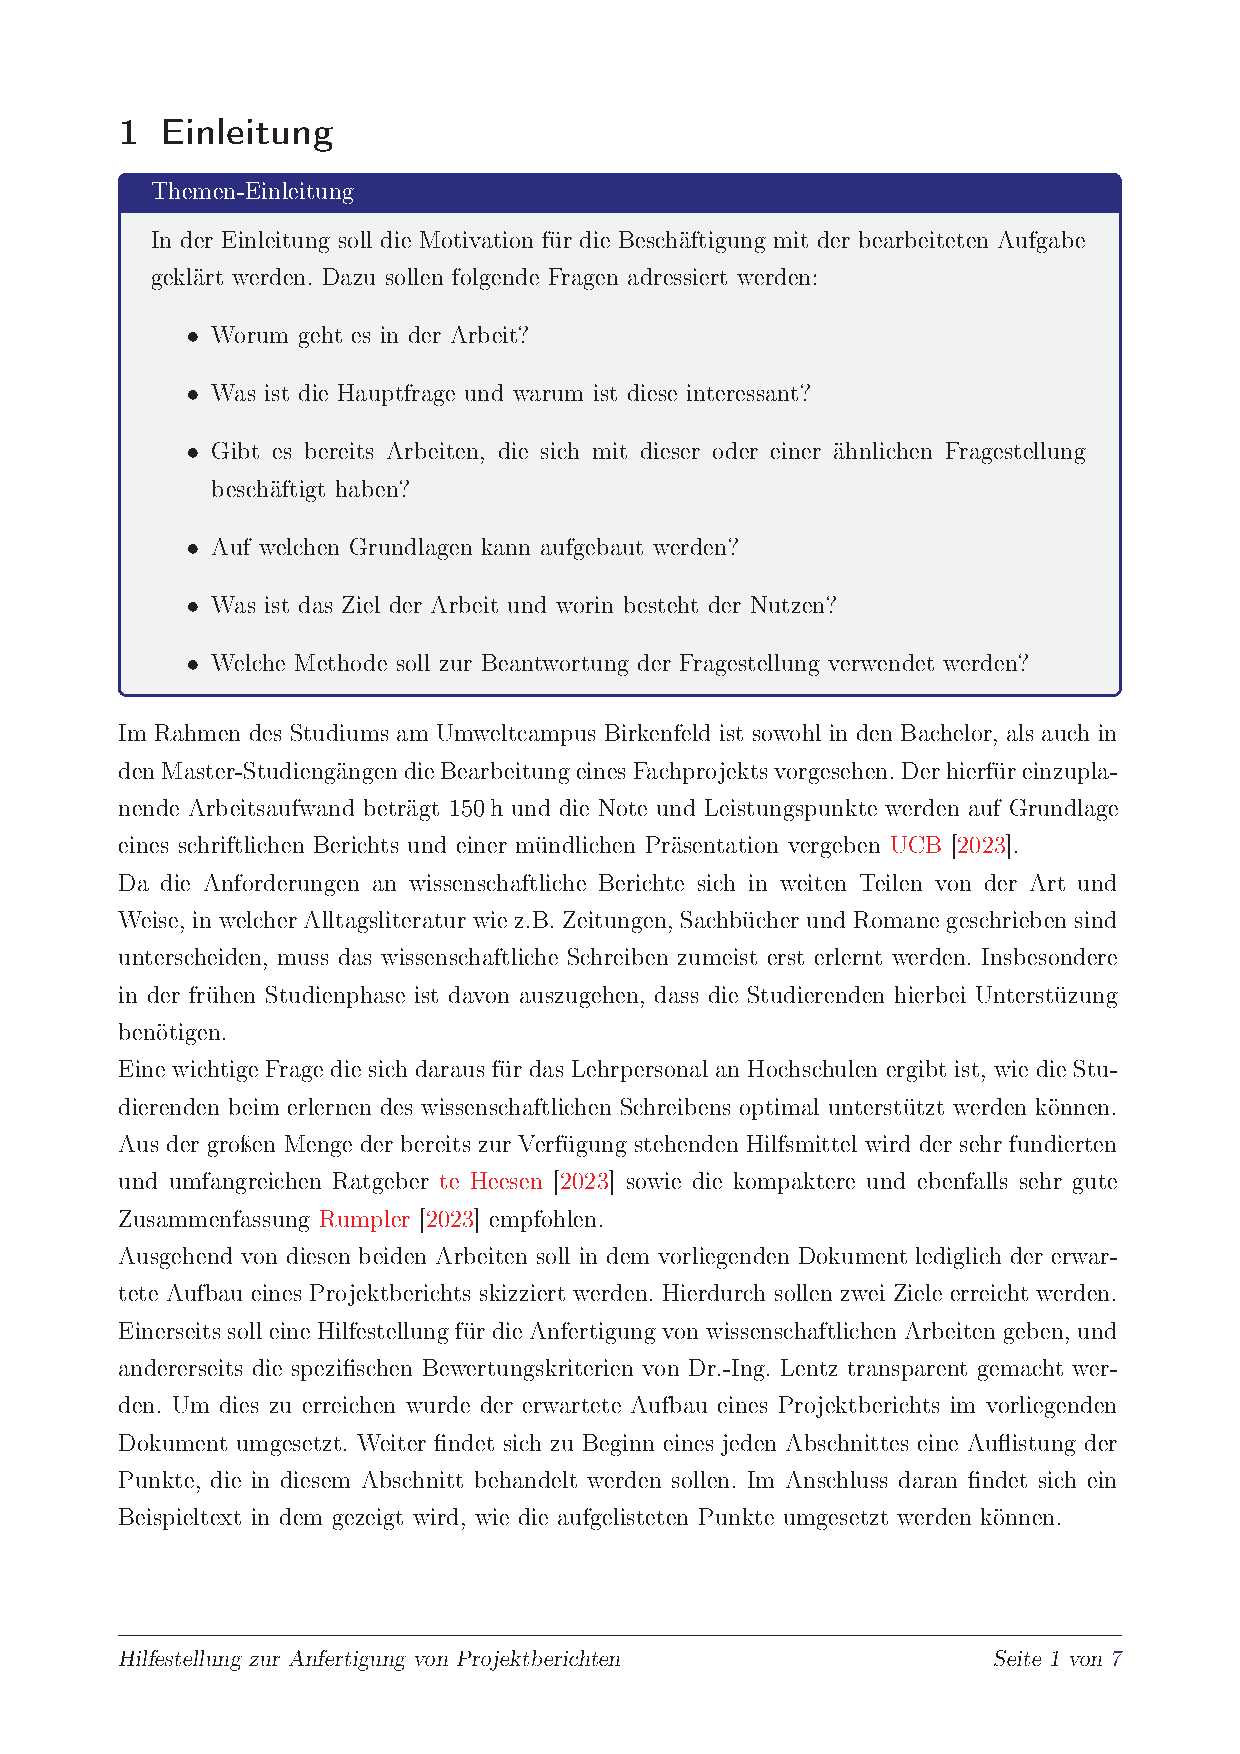
\includegraphics[page=1,scale=0.6,trim=2cmcm 12cm 2cm 3cm,clip]{Bilder//Aufbau.pdf}};
\node[above right = of fig.east,align=left,text=orange] (text1) {Punkte die behandelt\\ werden sollen};
\node[below right = of fig.east,align=left,yshift=-1.5cm,text=orange] (text2) {Textbeispiel};
\end{tikzpicture}
\caption{Darstellung des prinzipiellen Aufbaus eines Abschnitts in der Hilfestellung.}
\label{fig:seite}
\end{figure}
%
\par
Unter dem Kasten mit den zu behandelten Punkten findet sich ein Textbeispiel, in dem die Abarbeitung der Punkte erfolgt. 
Da in der Hilfestellung kein technisches Projekt beschrieben wird, sondern erläutert wird, wie ein Bericht aussehen soll, wirken die Textbeispiele leider manchmal etwas gekünstelt, was der Situation geschuldet ist. 
\par
Für die Erstellung der Hilfestellung wurde das  plattformunabhängige und kostenfreie Softwarepaket \LaTeX verwendet.
Nach einer gewissen Einarbeitungszeit lassen sich hiermit sehr systematisch und robust Dokumente mit ansprechendem Layout erzeugen, wobei eine besondere Stärke in der Darstellung von Formeln liegt.
Bei Interesse finden sich auf der Homepage des Verfassers zahlreiche Links zu Minimalbeispielen, die den Einstieg in die Verwendung von \LaTeX erleichtern.
Die Dateien welche zur Erstellung der Hilfestellung verwendet wurden, können Sie unter \url{https://github.com/lukaslentz/Bericht-Fachprojekt} ebenfalls herunterladen und weiterverwenden.
Obwohl \LaTeX also viele Vorzüge für das wissenschftliche Schreiben bietet, sind Sie natürlich frei in der Wahl des Textverarbeitungssystems, welches Sie zum Schreiben des Berichts verwenden wollen. 
%
